\documentclass[handout, 11pt]{beamer}
\usetheme{Goettingen}
\usepackage[utf8]{inputenc}
\usepackage{amsmath}
\usepackage{amsfonts}
\usepackage{amssymb}
\usepackage{graphicx}
\usepackage{hyperref}
\author{Alex Heilman}
\title{Spherical Harmonics, CG Coefficients, and CGCNN}

%\setbeamercovered{transparent} 
%\setbeamertemplate{navigation symbols}{} 
%\logo{} 
%\institute{} 
%\date{} 
%\subject{} 

\newenvironment{boxed2}
    {\begin{center}
    \begin{tabular}{|p{0.95\textwidth}|}
    \hline\\
    }
    { 
    \\\\\hline
    \end{tabular} 
    \end{center}
    }


\begin{document}

\begin{frame}
\titlepage
\end{frame}

%\begin{frame}
%\tableofcontents
%\end{frame}

\begin{frame}{Overview}

$\bullet$ Spherical Harmonics \pause $\rightarrow$ Just 2-parameter functions!\pause

\vspace{1cm}

$\bullet$ Clebsch-Gordon Coefficients \pause $\rightarrow$ Just look them up in a table! \pause

\vspace{1cm}

$\bullet$ An example of a Crystal Graph Convolutional Neural Network (CGCNN)

\end{frame}

\section{Spherical Harmonics}
\begin{frame}{Spherical Harmonics}
\begin{center}
JUST A NICE SET OF TWO-PARAMETER FUNCTIONS!
\end{center}
\end{frame}

\begin{frame}{Origin: Spherical Laplacian}
If you haven't seen differential equations before, don't worry! I just want you to see this in case it comes up again.

\pause

\begin{center}
Apply Laplace's equation to an arbitrary function in spherical coordinates:

\begin{align*}
\nabla^2 f(\phi,\theta,r) & = 0\\ \pause
\Bigg[
\frac{1}{r^2}\frac{\partial}{\partial r}\Big(r^2\frac{\partial}{\partial r}\Big)+\frac{1}{r^2\sin\theta}\frac{\partial}{\partial \theta}\Big(\sin\theta\frac{\partial}{\partial \theta}\Big)+\frac{1}{r^2\sin^2\theta}\frac{\partial^2}{\partial^2 \phi}\Bigg]f&=0\\
\end{align*}
\end{center}
\end{frame}

\begin{frame}{Origin: Spherical Laplacian cont.}\small
Now, we make the assumption (which works for Laplace's equation) that the solution is separable such that it is a product of simpler functions:  $f(\theta,\phi, r)=\Theta(\theta)\Phi(\phi)R(r)$.

\medskip

Then we may isolate the angular dependence into a function $Y_{\ell}^{m}(\theta,\phi)$, which satisfies:
$$\Bigg[\frac{1}{\sin\theta}\frac{\partial}{\partial \theta}\Big(\sin\theta\frac{\partial}{\partial \theta}\Big)+\frac{1}{\sin^2\theta}\frac{\partial^2}{\partial^2 \phi}\Bigg]Y^m_{\ell}=0$$
\pause


These functions, termed the spherical harmonics, take the form:
$$
Y_{\ell}^{m}(\theta,\phi)=C_{m\ell}P_{\ell}^m (\cos\theta)e^{-im\phi} 
$$

where $P^{m}_{\ell}(x)$ are the associated Legendre polynomials, and $C_{m\ell}$ is just some constant/normalization coefficient.

\medskip\pause

Note that their value is in general a complex number. Also note that $Y_{\ell}^m =0$ for $m>\ell$ and $m<\ell$, where $m$ and $\ell$ must be integers.\normalsize
\end{frame}

\begin{frame}{Origin: Irreducible Representation of SO(3)}
Spherical Harmonics also may be taken as the basis set for irreducible representations of the group of rotations in 3-space ($SO(3)$).

\vspace{.4cm}\pause

We can always decompose functions defined on a surface of a sphere as a linear combination of these spherical harmonics as below:

$$
f(\theta, \phi) = \sum_{\ell=0}^{\infty}\sum_{m=-\ell}^{m=\ell}c_{\ell, m}Y_{\ell}^m(\theta, \phi) 
$$

\end{frame}

\begin{frame}{Spherical Harmonics Practically}
Spherical harmonics are just two-dimensional functions!!!

\vspace{0.4cm}\pause

They have some nice properties  that make them indispensable for dealing with functions on the surface of spheres (they form an orthonormal basis). 

\vspace{0.4cm}\pause

A nice way to visualize them is to plot their magnitude as the radius in three dimensional space (where the input is the pair of angles $\theta, \phi$). See this ipython notebook to play with them: \url{https://alexheilman.com/products/ipy/spherical_harm_vis.ipy}
\end{frame}

\section{Clebsch-Gordon}
\begin{frame}{Tensor Products of SO(3)}
Say we want to describe the product of two spherical harmonics in terms of a third (equivalent to the product) spherical harmonic expansion. \small

$$
Y_{\ell_1}^{m_1}(\Omega)Y_{\ell_2}^{m_2}(\Omega)=\sum_{\ell_3, m_3}\sqrt{\frac{(2\ell_1+1)(2\ell_2+1)}{4\pi(2\ell_3+1)}}C^{\ell_3m_3}_{\ell_1m_1\ell_2m_2}C^{\ell_30}_{\ell_1 0\ell_2 0}Y_{\ell_3m_3}(\Omega)
$$
\normalsize

where $C^{LM}_{\ell_1m_1\ell_2m_2}$ are Clebsch-Gordon coefficients.

\medskip\pause

In physics, they're most often used for addition of angular momenta. In fact, this is the most common application of them. Hence, sometimes CG coefficients are often given the alternative notation:

$$
C^{LM}_{\ell_1m_1\ell_2m_2} = \langle  j_1m_1 j_2m_2\vert  L M  \rangle
$$
\end{frame}


\begin{frame}{CG Practically}
\begin{center}

They're just numbers.

\vspace{.5cm}

LOOK THEM UP IN A TABLE!
\end{center}
\end{frame}

\section{CGCNN}
\begin{frame}{Graphs (Not Plots of Functions)}

Graphs are mathematical objects. They're just sets of nodes and edges that connect two nodes.

\begin{center}

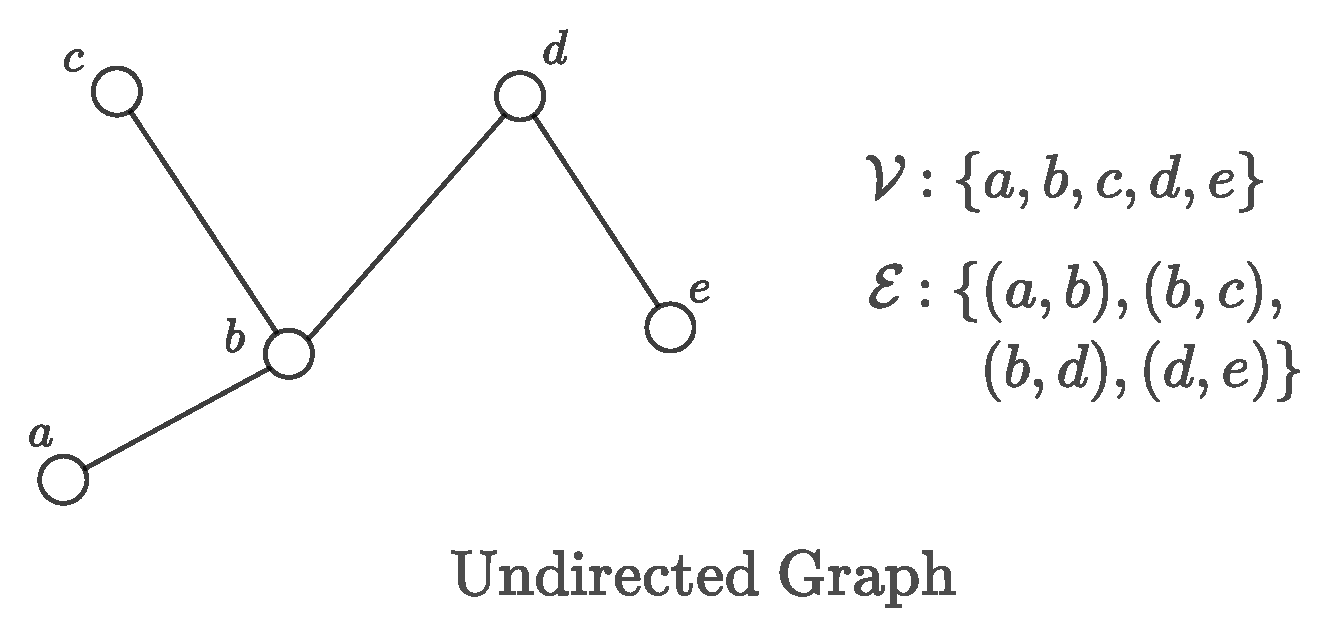
\includegraphics[scale=0.35]{undgraphex.pdf}

\end{center}

\end{frame}

\begin{frame}{Crystal Graphs}
Now, we'd like to encode crystalline structures as graphs and associate physical information with the graph elements:

\medskip

\begin{center}
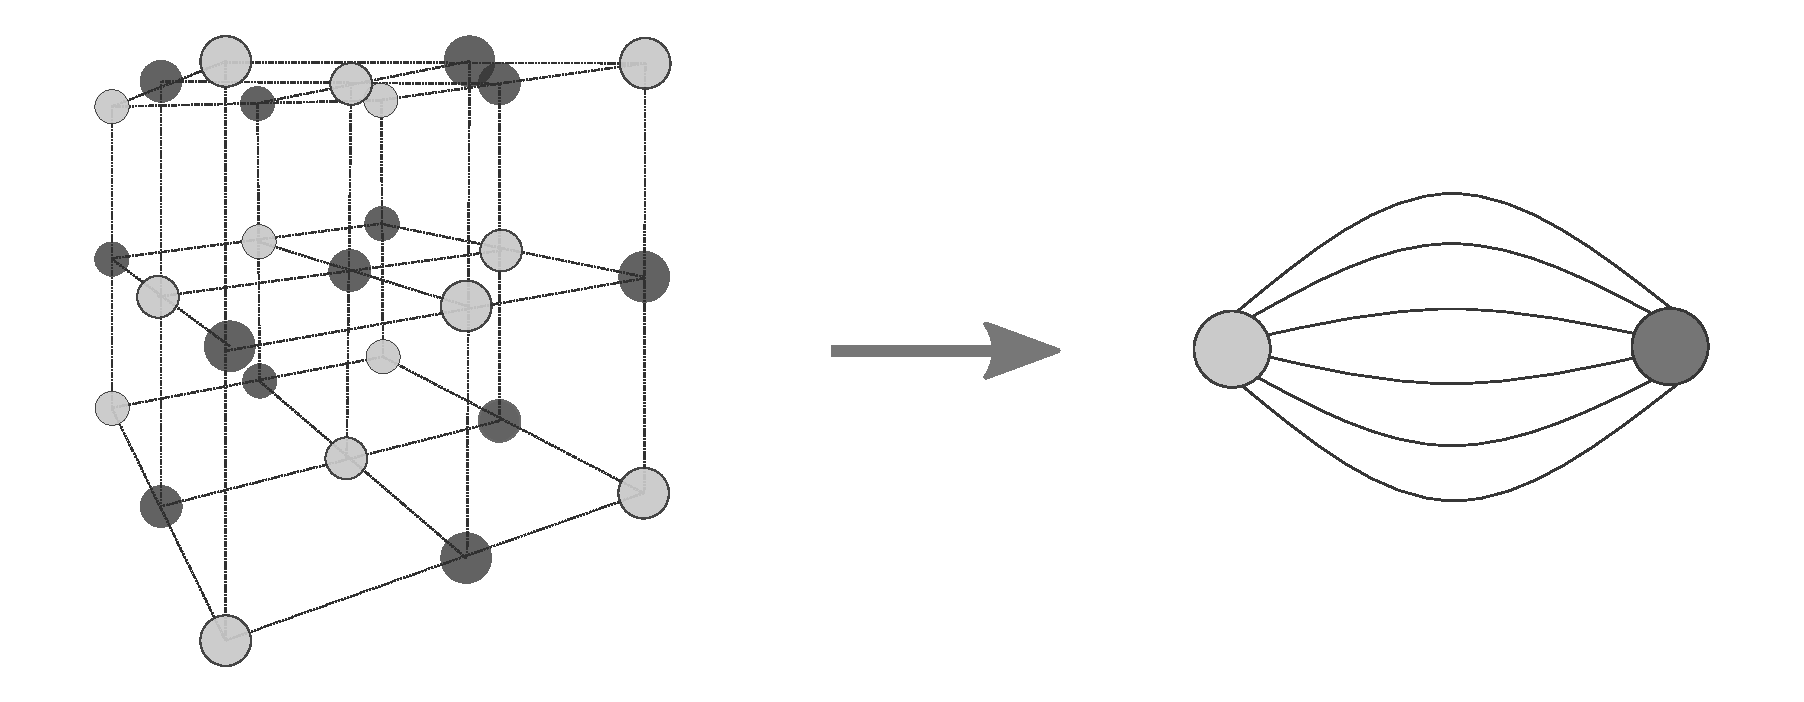
\includegraphics[scale=0.3]{crystalgraphintro.pdf}
\end{center}

\medskip

For an overview of the usual techniques, see \url{https://alexheilman.com/halfbaked/crystalgraphs}
\end{frame}

\begin{frame}{Graph Convolutional Neural Networks}
Graph neural networks act on and update the node features based upon the connectivity of the graph, while preserving the underlying graph structure. 


\vspace{1cm}

For a nice overview of basic graph networks and convolution see: 

\url{https://distill.pub/2021/gnn-intro/}

\url{https://distill.pub/2021/understanding-gnns/}
\end{frame} 


\begin{frame}{Machine Learning \& Materials Science}
Most state-of-the-art machine learning models applied to materials science utilize graph networks.

\vspace{1cm}

One of the original models is Tian Xie and Jeffrey Grossman's Crystal Graph Convolutional Neural Network (CGCNN). 


\end{frame}

\begin{frame}{CGCNN Architecture}
\begin{minipage}{.55\textwidth}
\begin{center}
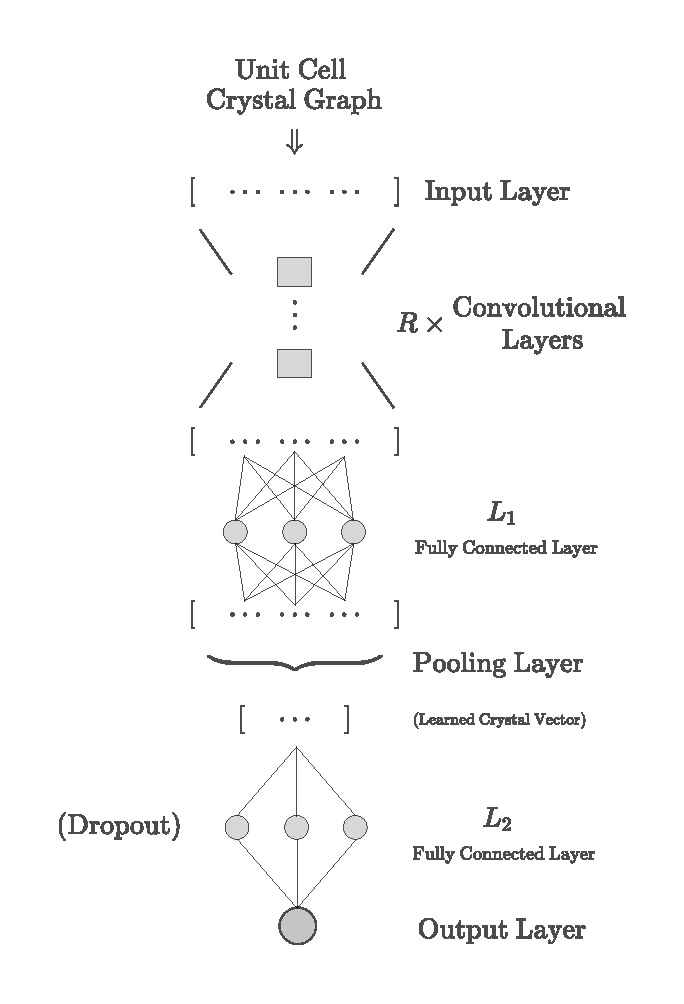
\includegraphics[scale=0.45]{cgcnn_arch.pdf}
\end{center}
\end{minipage}%
\begin{minipage}{0.45\textwidth}
A schematic of the basic CGCNN architecture is presented aside.

\vspace{0.7cm}

Note that both edge and node features are generally used, but node features are the only ones updated.

\vspace{0.7cm}

For the corresponding paper, see \url{https://link.aps.org/doi/10.1103/PhysRevLett.120.145301}.
\end{minipage}

\end{frame}
\end{document}